\chapter{列表和元组}
数据结构是以某种方式(如通过编号)组合起来的数据元素(如数、字符乃至其他数据结构)集合。在Python中,最基本的数据结构为序列(sequence)。序列中的每个元素都有编号,即其位置或索引,其中第一个元素的索引为0,第二个元素的索引为1,依此类推。从0开始指出相对于序列开头的偏移量,这显得更自然。同时可回绕到序列末尾,用负索引表示序列末尾元素的位置。

元组是一种特殊的序列,类似于列表,只是不能修改。
\section{序列概述}
Python内置了多种序列,本章重点讨论其中最常用的两种:列表和元组。另一种重要的序列是字符串,将在下一章更详细地讨论。

列表和元组的主要不同在于,列表是可以修改的,而元组不可以。这意味着列表适用于需要中途添加元素的情形,而元组适用于出于某种考虑需要禁止修改序列的情形。禁止修改序列通常出于技术方面的考虑,与Python的内部工作原理相关,这也是有些内置函数返回元组的原因所在。在你自己编写程序时,几乎在所有情况下都可使用列表来代替元组。一种例外情况是将元组用作字典键,在这种情况下,不能使用列表来代替元组,因为字典键是不允许修改的。

在需要处理一系列值时,序列很有用,序列还可以包含其他序列。

\begin{pyc}
edward = ["Edward Gumby", 42]
john = ["John Smith", 50]

database = [edward, john]
print(database)
\end{pyc}

\warning{
    Python支持一种数据结构的基本概念,名为容器(container)。容器基本上就是可包含其他对象的对象。两种主要的容器是序列(如列表和元组)和映射(如字典)。在序列中,每个元素都有编号,而在映射中,每个元素都有名称(也叫键)。映射将在\autoref{chapter04}详细讨论。有一种既不是序列也不是映射的容器,它就是集合(set),将在\autoref{chapter10}讨论。
}
\begin{figure}
    \centering
    \caption{Python中的主要容器(container)关系}
    \label{containerInPython}
    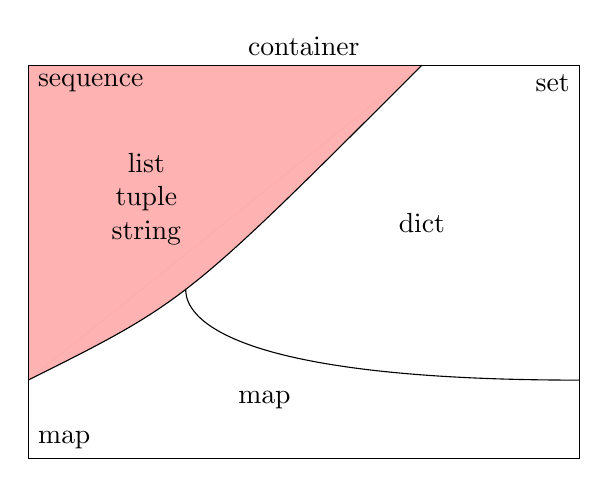
\begin{tikzpicture}
        \begin{scope}
        \fill[red, opacity=.3] (0, 1)--(0, 5)--(5, 5);
        \draw (0, 5) rectangle (7, 0);
        \fill[red, opacity=.3] (0, 1)..controls (2, 2)  and (2, 2).. (5, 5);
        \draw (0, 1)..controls (2, 2)  and (2, 2).. (5, 5);
        \draw (7, 1)..controls (2, 1)  and (2, 2).. (2, 2.16);
        \node[below left] at (7, 5){set};
        \node at (5, 3){dict};
        \node[below right] at (0, 5){sequence};
        \node[align=center] at (1.5, 3.3) {list\\ tuple\\string};
        \node[above right] at (0, 0){map};
        \node at (3, .75) {map};
        \node[above] at(3.5, 5){container};
        \end{scope}
        \end{tikzpicture}
\end{figure}

\section{通用的序列操作}
有几种操作适用于所有序列,包括索引、切片、相加、相乘和成员资格检查。另外,Python还提供了一些内置函数,可用于确定序列的长度以及找出序列中最大和最小的元素。
\warning{
    有一个重要的操作这里不会介绍,它就是迭代(iteration)。对序列进行迭代意味着对其每个元素都执行特定的操作。有关迭代的详细信息,请参阅\autoref{section5.5}节。
}
\subsection{索引(indexing)}
序列中的所有元素都有编号——从0开始递增。你可以这样通过编号来访问各个元素
\begin{pyc}
greeting = "Hello"
greeting[0] # "H"
\end{pyc}
这就是索引(indexing)。当你使用负数索引时,Python将从右(即从最后一个元素)开始往左数,因此-1是最后一个元素的位置\verb|greeting[-1]|。对于字符串字面量(以及其他的序列字面量),可直接对其执行索引操作,无需先将其赋给变量。这与先赋给变量再对变量执行索引操作的效果是一样的\verb|"Hello"[-1]|。
\begin{py}{索引操作示例}
months = ["January", "February", "March", "April", "May", "June",
    "July", "August", "September", "October", "November", "December"]
endings = ["st", "nd", "rd"] + 17 * ["th"] \
+ ["st", "nd", "rd"] + 7 * ["th"]\
+ ["st"]
year = input("Year: ")
month = input("Month: ")
day = input("Day: ")

month_number = int(month)
day_number = int(day)
month_name = months[month_number-1]
ordinal = day + endings[day_number-1]

print(month_name + " "+ordinal + ', ' + year)
\end{py}

\subsection{切片(slicing)}
除使用索引来访问单个元素外,还可使用切片(slicing)来访问特定范围内的元素。为此,可使用两个索引,并用冒号分隔:
\begin{pyc}
tag = "<a href='http://www.python.org'>Python web site</a>"
tag[9:30]  # 'http://www.python.org'

tag[32:-4]  # 'Python web site'
\end{pyc}

切片适用于提取序列的一部分,其中的编号非常重要:第一个索引是包含的第一个元素的编号,但第二个索引是切片后余下的第一个元素的编号。简而言之,你提供两个索引来指定切片的边界,其中第一个索引指定的元素包含在切片内,但第二个索引指定的元素不包含在切片内。
\begin{pyc}
numbers = [1, 2, 3, 4, 5, 6, 7, 8, 9, 10]
numbers[3:6]  # [4, 5, 6]
numbers[0:1]  # [1]
\end{pyc}

\subsubsection{绝妙的简写}
假设你想要访问前述列表的最后三个元素,显然可以明确地指定\verb|numbers[7:10]|。如果要从列表末尾开始数,可使用负数索引\verb|numbers[-3:-1]|,然而,这样好像无法包含最后一个元素。如果使用索引0,即到达列表末尾后再前进一步所处的位置,结果将如何呢?\verb|numbers[-3:0] # []|。\textbf{执行切片操作时,如果第一个索引指定的元素位于第二个索引指定的元素后面(在这里,倒数第3个元素位于第1个元素后面),结果就为空序列。}好在你能使用一种简写:如果切片结束于序列末尾,可省略第二个索引\verb|numbers[-3:]|。同样,如果切片始于序列开头,可省略第一个索引\verb|numbers[:3]|。实际上,要复制整个序列,可将两个索引都省略\verb|numbers[:]|。

\begin{pyc}
url = input("Please enter the URL: ")
domain = url[11:-4]
print("Domain name: " + domain)
\end{pyc}

\subsubsection{更大的步长}
执行切片操作时,你显式或隐式地指定起点和终点,但通常省略另一个参数,即步长。在普通切片中,步长为1。如果指定的步长大于1,将跳过一些元素。显式地指定步长时,也可使用前述简写。当然,步长不能为0,否则无法向前移动,但可以为负数,即从右向左提取元素。步长为负数时,第一个索引必须比第二个索引大。可能有点令人迷惑的是,当你省略起始和结束索引时,Python竟然执行了正确的操作:步长为正数时,它从起点移到终点,而步长为负数时,它从终点移到起点。

\begin{pyc}
numbers[0:10:1]
numbers[0:10:2]  # [1, 3, 5, 7, 9]

numbers[3:6:3]  # [4]

numbers[8:3:-1]  # [9, 8, 7, 6, 5]
numbers[10:0:-1]  # [10, 9, 8, 7, 6, 5, 4, 3, 2]
numbers[:5:-2]  # [10, 8]
numbers[5::-2]  # [10, 8]
\end{pyc}

\subsection{序列相加}
可使用加法运算符来拼接序列。一般而言,不能拼接不同类型的序列。
\begin{pyc}
[1, 2, 3] + [4, 5, 6]  # [1, 2, 3, 4, 5, 6]
"Hello, " + "Python!"  # 'Hello, Python!'
# TypeError: can only concatenate list (not "str") to list
[1, 2, 3] + "Python!"
\end{pyc}

\subsection{乘法}
将序列与数x相乘时,将重复这个序列x次来创建一个新序列:
\begin{pyc}
"Python" * 5  # 'PythonPythonPythonPythonPython'
[42] * 10  # [42, 42, 42, 42, 42, 42, 42, 42, 42, 42]
\end{pyc}
\subsubsection{None、空列表和初始化}
空列表是使用不包含任何内容的两个方括号([])表示的。然而,在有些情况下,你可能想使用表示“什么都没有”的值,如表示还没有在列表中添加任何内容。在这种情况下,可使用None。在Python中,None表示什么都没有。因此,要将列表的长度初始化为10,可像下面这样做:
\begin{pyc}
sequence = [None] * 10
print(sequence)  # [None, None, None, None, None, None, None, None, None, None]
\end{pyc}

\begin{py}{序列(字符串)乘法运算示例}
sentence = input("Sentence: ")
screen_width = 80
text_width = len(sentence)
box_width = text_width + 6
left_margin = (screen_width - text_width) // 2
print()
print(" " * left_margin + "+" + "-" * (box_width - 2) + "+")
print(" " * left_margin + "|  " + " " * text_width + "  |")
print(" " * left_margin + "|  " + sentence + "  |")
print(" " * left_margin + "|  " + " " * text_width + "  |")
print(" " * left_margin + "+" + "-" * (box_width - 2) + "+")
print()
\end{py}

\subsubsection{成员资格}
要检查特定的值是否包含在序列中,可使用运算符\verb|in|。它检查是否满足指定的条件,并返回相应的值:满足时返回True,不满足时返回False。这样的运算符称为布尔运算符,而前述真值称为布尔值。
\begin{pyc}
permissions = "rw"
"w" in permissions  # True
"x" in permissions  # False
user = ["mlh", "foo", "bar"]
input("Enter your user name: ") in user
subject = '$$ Get rich now !!!'
"$$" in subject  # True
\end{pyc}

\warning{
    相比于其他示例,检查字符串是否包含\texttt{'\$\$'}的示例稍有不同。一般而言,运算符in检查指定的对象是否是序列(或其他集合)的成员(即其中的一个元素),但对字符串来说,只有它包含的字符才是其成员或元素。事实上,在较早的Python版本中,只能对字符串执行这种成员资格检查——确定指定的字符是否包含在字符串中,但\textbf{现在可使用运算符in来检查指定的字符串是否为另一个字符串的子串}。
}

\begin{py}{序列成员资格示例}
database = [
    ['albert', '1234'],
    ['dilbert', '4242'],
    ['smith', '7523'],
    ['jones', '9753']
]
username = input('User name: ')
pin = input("PIN code: ")
if [username, pin] in database:
    print("Access Granted")
\end{py}

特定值的样式或者类型应该与判定序列中元素的样式或者类型相同,也就是示例中为什么使用列表作为特定值的原因。

\subsubsection{长度、最大值和最小值}
内置函数len、min和max很有用,其中函数len返回序列包含的元素个数,而min和max分别返回序列中最小和最大的元素。
\begin{pyc}
numbers = [100, 34, 678]
len(numbers)  # 3
max(numbers)  # 678
min(numbers)  # 34

max(2, 3)  # 3
min(9, 3, 2, 5)  # 2
\end{pyc}
最后两行代码调用max和min时指定的实参并不是序列,而直接将数作为实参。

\section{列表:Python的主力}
\subsection{函数list}
鉴于不能像修改列表那样修改字符串,因此在有些情况下使用字符串来创建列表很有帮助。 为此,可使用函数list\footnote{它实际上是一个类,而不是函数。}。
\begin{pyc}
list("Hello")  # ['H', 'e', 'l', 'l', 'o']
\end{pyc}
\warning{
    请注意,可将任何序列作为list的参数。
}

要将字符列表(如前述代码中的字符列表)转换为字符串,可使用下面的表达式:\verb|''.join(somelist)|,其中somelist是要转换的列表。
\subsection{基本的列表操作}
可对列表执行所有的标准序列操作,如索引、切片、拼接和相乘,但列表的有趣之处在于它是可以修改的。本节将介绍一些修改列表的方式:给元素赋值、删除元素、给切片赋值以及使用列表的方法。
\subsubsection{给元素赋值}
修改列表很容易,只需使用索引表示法给特定位置的元素赋值,如\verb|x[1] = 2|。
\begin{pyc}
x = [1] * 3
x[1] = 2
x  # [1, 2, 1]
\end{pyc}

\warning{
    不能给不存在的元素赋值,因此如果列表的长度为2,就不能给索引为100的元素赋值。要这样做,列表的长度至少为101。
}
\subsubsection{删除元素}
从列表中删除元素也很容易,只需使用del语句即可。
\begin{pyc}
names = ["Alice", "Beth", "Cecil", "Dee-Dee", "Earl"]
del names[2]
names  # ['Alice', 'Beth', 'Dee-Dee', 'Earl']
\end{pyc}
\subsubsection{给切片赋值}
切片是一项极其强大的功能,而能够给切片赋值让这项功能显得更加强大。
\begin{pyc}
name = list("Perl")
name  # ['P', 'e', 'r', 'l']
name[2:] = list("ar")
name  # ['P', 'e', 'a', 'r']
\end{pyc}

从上述代码可知,可同时给多个元素赋值。你可能认为,这有什么大不了的,分别给每个元素赋值不是一样的吗?确实如此,但\important{通过使用切片赋值,可将切片替换为长度与其不同的序列}。
\begin{pyc}
name = list("Perl")
name[1:] = list("ython")
name  # ['P', 'y', 't', 'h', 'o', 'n']
\end{pyc}

使用切片赋值还可在不替换原有元素的情况下插入新元素。你可采取相反的措施来删除切片。
\begin{pyc}
numbers = [1, 5]
numbers[1:1] = [2, 3, 4]
numbers  # [1, 2, 3, 4, 5]

numbers[1:4] = []
numbers  # [1, 5]
\end{pyc}

\subsection{列表方法}
方法是与对象(列表、数、字符串等)联系紧密的函数。通常,像下面这样调用方法:

\verb|object.method(arguments)|

方法调用与函数调用很像,只是在方法名前加上了对象和句点。
\subsubsection{append}
方法 append 用于将一个对象附加到列表末尾。

\begin{pyc}
lst = [1, 2, 3]
lst.append(4)
lst  # [1, 2, 3, 4]
\end{pyc}
你可能还记得,list是一个内置函数\footnote{实际上,从Python 2.2起,list就是类型,而不是函数了(tuple和str亦如此)。},如果我将前述列表命名为list,就无法调用这个函数。在特定的应用程序中,通常可给列表选择更好的名称。

\warning{
    另外请注意,与其他几个类似的方法一样,append也就地修改列表。这意味着它不会返回修改后的新列表,而是直接修改旧列表。
}
\begin{pyc}
lst = [1, 2, 3]
ret = lst.append(4)
print(ret)  # None
\end{pyc}

\subsubsection{clear}
方法 clear 就地清空列表的内容,列表仍然存在,称为空列表。类似于切片赋值语句\verb|lst[:] = []|。
\begin{pyc}
lst = [1, 2, 3]
lst.clear()
lst  # []
\end{pyc}
\subsubsection{copy}
方法 copy 复制列表,常规复制只是将另一个名称关联到列表。
\begin{pyc}
a = [1, 2, 3]
b = a
b[1] = 4
a  # [1, 4, 3]
\end{pyc}
要让a和b指向不同的列表,就必须将b关联到a的副本。
\begin{pyc}
a = [1, 2, 3]
b = a.copy()
b[1] = 4
a  # [1, 2, 3]
\end{pyc}
这类似于使用\verb|a[:]|或\verb|list(a)|,它们也都复制a。
\begin{pyc}
a = [1, 2, 3]
b = a[:]
b[1] = 4
a  # [1, 2, 3]

a = [1, 2, 3]
b = list(a)
b[1] = 4
a  # [1, 2, 3]
\end{pyc}
\subsubsection{count}
方法 count 计算指定的元素在列表中出现了多少次,最检索最外层的列表元素,嵌套的对象不会检索。
\begin{pyc}
['to', 'be', 'or', 'not', 'to', 'be'].count('to')  # 2
x = [[1, 2], 1, 1, [2, 1, [1, 2]]]
x.count(1)  # 2
x.count([1, 2])  # 1
\end{pyc}

\subsubsection{extend}
方法extend让你能够同时将多个值附加到列表末尾,为此可将这些值组成的序列作为参数提供给方法extend。换而言之,你可使用一个列表来扩展另一个列表。这可能看起来类似于拼接,但存在一个重要差别,那就是将修改被扩展的序列(这里是a)。在常规拼接中,返回的是一个全新的序列。

\begin{pyc}
a = [1, 2, 3]
b = [4, 5, 6]
a.extend(b)
a  # [1, 2, 3, 4, 5, 6]

a = [1, 2, 3]
a + b
a  # [1, 2, 3] 
\end{pyc}
鉴于常规拼接必须使用a和b的副本创建一个新列表,因此如果你要获得类似于\verb|a = a + b|的效果,拼接的效率将比extend低。另外,拼接操作并非就地执行的,即它不会修改原来的列表。要获得与extend相同的效果,可将列表赋给切片,但可读性不是很高。

\begin{pyc}
a = [1, 2, 3]
b = [4, 5, 6]
a[len(a):] = b
a  # [1, 2, 3, 4, 5, 6]
\end{pyc}

\subsubsection{index}
方法 index 在列表中\important{查找指定值第一次出现的索引},如果查找不存在的值就会报错,最好使用成员资格进行判断在执行index方法。
\begin{pyc}
knights = ['We', 'are', 'the', 'knights', 'who', 'say', 'ni']
knights.index('who')  # 4
knights.index('Stephen')  # ValueError: 'Stephen' is not in list
\end{pyc}

\subsubsection{insert}
方法insert用于将一个对象插入列表。也可以切片赋值来获得与insert一样的效果,但可读性根本无法与使用insert媲美。
\begin{pyc}
numbers = [1, 2, 3, 5, 6, 7]
numbers.insert(3, 'four')
numbers  # [1, 2, 3, 'four', 5, 6, 7]

numbers = [1, 2, 3, 5, 6, 7]
numbers[3:3] = ['four']
numbers  # [1, 2, 3, 'four', 5, 6, 7]
\end{pyc}

\subsubsection{pop}
方法 pop 从列表中删除一个元素(末尾为最后一个元素),并返回这一元素。\important{pop是唯一既修改列表又返回一个非None值的列表方法。}
\begin{pyc}
x = [1, 2, 3]
x.pop()  # 3
x  # [1, 2]
x.pop(0)
x  # [2]
\end{pyc}

使用pop可实现一种常见的数据结构——栈(stack)。栈就像一叠盘子,你可在上面添加盘子,还可从上面取走盘子。最后加入的盘子最先取走,这被为后进先出(LIFO)。

push和pop是大家普遍接受的两种栈操作(加入和取走)的名称。Python没有提供push,但可使用append来替代。方法pop和append的效果相反,因此将刚弹出的值压入(或附加)后,得到的栈将与原来相同。

\begin{pyc}
x = [1, 2, 4]
x.append(x.pop())
x  # [1, 2, 4]
\end{pyc}

要创建先进先出(FIFO)的队列,可使用insert(0, ...)代替append。另外,也可继续使用append,但用pop(0)替代pop()。一种更佳的解决方案是,使用模块collections中的deque。有关这方面的详细信息,请参阅\autoref{chapter10}。

\subsubsection{remove}
方法 remove 用于删除第一个为指定值的元素,删除不存在的元素会报错。

\begin{pyc}
x = ['to', 'be', 'or', 'not', 'to', 'be']
x.remove('be')
x  # ['to', 'or', 'not', 'to', 'be']
x.remove('bee')  # list.remove(x): x not in list
\end{pyc}


\subsubsection{reverse}
方法 reverse 按相反的顺序排列列表中的元素,注意到reverse修改列表,但不返回任何值。

\begin{pyc}
x = [7, 9, 3]
x.reverse()
x  # [3, 9, 7]
\end{pyc}

\warning{
    如果要按相反的顺序迭代序列,可使用函数reversed。这个函数不返回列表,而是返回一个迭代器(迭代器将在第9章详细介绍)。你可使用list将返回的对象转换为列表。
}

\subsubsection{sort}
方法sort用于对列表就地排序,\important{就地排序意味着对原来的列表进行修改,使其元素按顺序排列,而不是返回排序后的列表的副本}。

\begin{pyc}
x = [4, 6, 2, 1, 7, 9]
x.sort()
x  # [1, 2, 4, 6, 7, 9]
\end{pyc}

前面介绍了多个修改列表而不返回任何值的方法,需要强调sort的行为也是这样的,因为这种行为给很多人都带来了困惑。在需要排序后的列表副本并保留原始列表不变时,通常会遭遇这种困惑。

\begin{py}{一种错误的排序且保留之前列表}
x = [4, 6, 2, 1, 7, 9]
y = x.sort()
x  # [1, 2, 4, 6, 7, 9]
print(y)  # None
\end{py}
鉴于sort修改x且不返回任何值,最终的结果是x是经过排序的,而y包含None。为实现前述目标,正确的方式之一是先将y关联到x的副本,再对y进行排序。

为获取排序后的列表的副本,另一种方式是使用函数sorted,这个函数可用于任何序列,但\important{总是返回一个列表}。

\subsubsection{高级排序}
方法sort接受两个可选参数:key和reverse。参数key类似于参数cmp:你将其设置为一个用于排序的函数。然而,不会直接使用这个函数来判断一个元素是否比另一个元素小,而是使用它来为每个元素创建一个键,再根据这些键对元素进行排序。

\begin{pyc}
x = ['aardvark', 'abalone', 'acme', 'add', 'aerate']
x.sort(key=len)
x  # ['add', 'acme', 'aerate', 'abalone', 'aardvark']
\end{pyc}

另一个关键字参数reverse,只需将其指定为一个真值(True或False),以指出是否要按相反的顺序对列表进行排序。
\begin{pyc}
x = ['aardvark', 'abalone', 'acme', 'add', 'aerate']
x.sort(key=len, reverse=True)
x  # ['aardvark', 'abalone', 'aerate', 'acme', 'add']
\end{pyc}

如果你想更深入地了解排序,可以参阅文章“\href{https://wiki.python.org/moin/HowTo/Sorting}{Sorting Mini-HOW TO}”

\section{元组:不可修改的序列}
与列表一样,元组也是序列,唯一的差别在于元组是不能修改的。元组语法很简单,只要将一些值用逗号分隔,就能自动创建一个元组。
\begin{itemize}
    \item 元组还可用圆括号括起(这也是通常采用的做法)。
    \item 空元组用两个不包含任何内容的圆括号表示。
    \item 只有一个值,也必须在它后面加上逗号,否则就是个数字。
    \item 函数tuple的工作原理与list很像:它将一个序列作为参数,并将其转换为元组。如果参数已经是元组,就原封不动地返回它。
\end{itemize}

\begin{pyc}
1, 2, 3  # (1, 2, 3)
(1, 2, 3)  # (1, 2, 3)
()  # ()
42,  # (42,)

tuple([1, 2, 4])  # (1, 2, 4)
tuple('abc')  # ('a', 'b', 'c')
tuple((1, 2, 3))  # (1, 2, 3)
\end{pyc}

元组的切片也是元组,就像列表的切片也是列表一样。为何要熟悉元组呢?原因有以下两个。
\begin{itemize}
    \item 它们用作映射中的键(以及集合的成员),而列表不行。
    \item 有些内置函数和方法返回元组,这意味着必须跟它们打交道。只要不尝试修改元组,与元组“打交道”通常意味着像处理列表一样处理它们(需要使用元组没有的index和count等方法时例外)。
\end{itemize}
\section{小结}
\begin{dinglist}{42}
    \item \important{序列}:序列是一种数据结构,其中的元素带编号(编号从0开始)。\important{列表、字符串和元组都属于序列,其中列表是可变的(你可修改其内容),而元组和字符串是不可变的(一旦创建,内容就是固定的)}。要访问序列的一部分,可使用切片操作:提供两个指定切片起始和结束位置的索引。要修改列表,可给其元素赋值,也可使用赋值语句给切片赋值。
    \item \important{成员资格}:要确定特定的值是否包含在序列(或其他容器)中,可使用运算符in。将运算符in用于字符串时情况比较特殊——这样可查找子串。
    \item 方法:一些内置类型(如列表和字符串,但不包括元组)提供了很多有用的方法。方法有点像函数,只是与特定的值相关联。方法是面向对象编程的一个重要方面
\end{dinglist}

\subsection{本章函数汇总}
\begin{table}
    \caption{列表与元组函数}
    \begin{tabularx}{\textwidth}{lXl}
        \hline
        函数名    & 说明           & 返回值  \\
        \hline
        append & 将一个对象附加到列表末尾 & None \\
        clear  & 就地清空列表内容     &      \\
        \hline
    \end{tabularx}
\end{table}